% `template.tex', a bare-bones example employing the AIAA class.
%
% For a more advanced example that makes use of several third-party
% LaTeX packages, see `advanced_example.tex', but please read the
% Known Problems section of the users manual first.
%
% Typical processing for PostScript (PS) output:
%
%  latex template
%  latex template   (repeat as needed to resolve references)
%
%  xdvi template    (onscreen draft display)
%  dvips template   (postscript)
%  gv template.ps   (onscreen display)
%  lpr template.ps  (hardcopy)
%
% With the above, only Encapsulated PostScript (EPS) images can be used.
%
% Typical processing for Portable Document Format (PDF) output:
%
%  pdflatex template
%  pdflatex template      (repeat as needed to resolve references)
%
%  acroread template.pdf  (onscreen display)
%
% If you have EPS figures, you will need to use the epstopdf script
% to convert them to PDF because PDF is a limmited subset of EPS.
% pdflatex accepts a variety of other image formats such as JPG, TIF,
% PNG, and so forth -- check the documentation for your version.
%
% If you do *not* specify suffixes when using the graphicx package's
% \includegraphics command, latex and pdflatex will automatically select
% the appropriate figure format from those available.  This allows you
% to produce PS and PDF output from the same LaTeX source file.
%
% To generate a large format (e.g., 11"x17") PostScript copy for editing
% purposes, use
%
%  dvips -x 1467 -O -0.65in,0.85in -t tabloid template
%
% For further details and support, read the Users Manual, aiaa.pdf.


% Try to reduce the number of latex support calls from people who
% don't read the included documentation.
%
\typeout{}\typeout{If latex fails to find aiaa-tc, read the README file!}
%


\documentclass[]{aiaa-tc}% insert '[draft]' option to show overfull boxes
\usepackage{amssymb}
\usepackage{amsmath}
\usepackage{svg} 

 \title{An Open-Source Reaction Wheel System for Oregon's First Satellite}

 \author{
  Jeremy A. Louke%
  	\thanks{Student BScME, Maseeh College of Engineering, Portland State University, Student Member.}\\
  {\normalsize\itshape
   Portland State Aerospace Society, Portland, OR, 97201}\\
  \and
  Erin S. Schmidt% 
  	\thanks{Student MSME, Maseeh College of Engineering, Portland State University, Student Member. esch2@pdx.edu} \ \
  Calvin J. Young\thanksibid{1}\\
  {\normalsize\itshape
  Portland State University, Portland, OR, 97201}
 }

 % Data used by 'handcarry' option if invoked
 \AIAApapernumber{YEAR-NUMBER}
 \AIAAconference{Conference Name, Date, and Location}
 \AIAAcopyright{\AIAAcopyrightD{YEAR}}

 % Define commands to assure consistent treatment throughout document
 \newcommand{\eqnref}[1]{(\ref{#1})}
 \newcommand{\class}[1]{\texttt{#1}}
 \newcommand{\package}[1]{\texttt{#1}}
 \newcommand{\file}[1]{\texttt{#1}}
 \newcommand{\BibTeX}{\textsc{Bib}\TeX}

\begin{document}

\maketitle

\begin{abstract}
Portland State University is developing Oregon's first orbital satellite, a 2U CubeSat, dubbed Oresat. This CubeSat will use a reaction wheel system for attitude control and pointing of the onboard low-gain antenna. Details of the development of the reaction wheel ground test article, and its controller, are presented here. Finally, preliminary results of attitude control testing conducted in the brief (2.1 s) free-fall environment of Portland State University's Dryden Drop Tower are presented here. 
\end{abstract}

\section*{Nomenclature}

\begin{center}
\parbox{0cm}
{\begin{tabbing}
  XXX \= \kill% this line sets tab stop
  $M_0^{+ \circlearrowleft}$ \qquad Moment in the x-axis (N m)\\
  $T^0$ \qquad Torque (N m)\\
  $\theta$ \qquad Angular position (${}^{\circ}$)\\
  $\dot{\theta}$ \qquad Angular velocity(${}^{\circ}/s$)\\ 
  $\ddot{\theta}$ \qquad Angular velocity(${}^{\circ}/s^2$) \\
  $I$ \qquad Moment of Inertia (N $\textrm{m}^2$)\\
  $b$ \qquad Damping Coefficient (N s/m)\\ 
  $G$ \qquad Spring Coefficient (N/m)\\
  $COTS$ \qquad Commercial Off-The Shelf\\
  $FDM$ \qquad Fused Deposition Modeling\\
  $IMU$ \qquad Inertial Measurement Unit\\
  $PWM$ \qquad Pulse Width Modulation\\ \\
  \textit{Subscripts}\\
  $x$ \qquad Index for Cartesian axes \\
  $rw$\qquad Reaction Wheel\\
  $n$ \qquad Motor Index\\
  $A, B, C, D$ \qquad Indices for Motors A, B, C, and D\\
 \end{tabbing}}
 \end{center}
 
\section{Introduction}
Small educational satellites have been launched by dozens of universities around the United States as part of NASA’s CubeSat Launch Initiative (CLSI), especially under the auspices of the Educational Launch of Nanosatellites (ELaNa) program. As of 2015 CubeSats from 29 states have flown under the program, however the great state of Oregon has yet to join their ranks\cite{Mahoney:15bk}. During the summer of 2015 the Oresat project was initiated by the Portland State Aerospace Society (PSAS) to rectify this situation. PSAS is an engineering student organization and citizen science project located at Portland State University dedicated to developing low-cost, open-source, and open-hardware high-powered rockets and avionics systems with special interests in venture class launch vehicle technologies and nanosatellites\cite{PSAS:15bk}.\\

The Oresat satellite will follow the ``2U" CubeSat standard \cite{Cubesat:14bk}. A CAD render of the Oresat concept is pictured in Figure \ref{fig:oresat}. The primary objectives of the project are to test several subsystems in the environment of a 400 km circular Low Earth Orbit: the ``Low Gain Radio (LGR)" communication board and the highly tolerant ``System Controller" board. The LGR is the main low-gain radio system based on a 436 MHz radio system using the MKW01Z128 microcontroller with built in sub-1GHz radio. The System Controller is being designed expressly for the space environment, and will include some measure of fault-tolerance and radiation hardening.

The secondary mission goal is to run an educational outreach project in the state of Oregon. Called ``DxWiFi", after the Amateur Radio ``Dx" code for distance, OreSat will broadcast a live video feed from space to the ground using the standard 2.4 GHz  802.11b ``WiFi" protocol. DxWiFi ground stations will be built by Oregon high schools using 3D printers, common-off-the-shelf WiFi adapter cards, and existing augmented reality cellphone apps that track satellites.

A severely power limited ($\sim$ 1 W) S-band downlink from LEO unfortunately requires high gain antennas, both on the ground and on the space vehicle. However, in order to minimize required deployables on the space vehicle, and to provide for the general simplicity of design, construction, and operation of future ground stations, we chose a 16 turn Helical with approximately 15 dBi gain. This gives a relatively broad beam width antenna, requiring pointing, but only on the order of a 5-10 degrees. Since nadir pointing will only allow a few seconds of data link, Oresat must "point and stare" at a ground station that has requested to download video. This degrees-per-second slew of the antenna (and camera) requires rapid pointing changes that magnetorquers simply can not provide. Following from this is the need for a robust system to provide attitude control for Oresat attitude control system. PSAS has selected a reaction wheel based system to provide attitude control for Oresat. Per PSAS’s open-source mandate all (non-ITAR) project development deliverables are being made publicly available under a GNU GPL v2 license\cite{Oresat:15bk}. It is hoped by the authors, and the members of PSAS that the discourse around educational CubeSats and their design will be elevated by making the information for this project publicly available.

\begin{figure}[h!]
  \centering
  \includegraphics[width=0.3\linewidth]{2U_CubeSat_V0o3.PNG}
  \caption{Speculative mockup in SolidWorks of the Oresat chassis.}
  \label{fig:oresat}
\end{figure}

\section{Concept Definition}
	Angular rate and pointing precision requirements for the flight attitude control system are determined from orbital parameters (likely those offered by Nanoracks deployment from the ISS) and the expected performance of the PSAS DxWiFi telemetry system. The ground test article is a proof of concept and uses inexpensive COTS DC brushless motors which are significantly more powerful than those required for the flight use case. The ground test article is broadly similar in design to the flight system, for example by using 4 momentum-wheels in a pyramid configuration for added redundancy and on-orbit mission assurance. Such a design is similar one recently developed for a master's thesis project at California Polytechnic State University San Luis Obispo\cite{Logan:08bk}. A magnetorquer will be used to periodically dump accumulated momentum into the Earth's magnetic field. The principle difference between the ground test and flight designs is that the ground test article uses the 1U form factor whereas Oresat will be 2U.

\section{Design and Fabrication}
	The Oresat reaction wheel system chassis was developed using rapid prototyping techniques over a short time period (approximately 8 weeks). This approach enables rapid design iteration cycles. A mockup 1U CubeSat structure was drafted in SolidWorks CAD, and fabricated using a FDM 3D printer. Mounted on the 3D-printed chassis are the 4X DC brushless motors, a 4-cell Li-Po battery pack, IMU shield, Intel Edison microcontroller and accompanying Arduino breakout. This `ground' test article is shown in Figure \ref{fig:rcs}. As previously noted there are several departures in the design of the ground test article from the flight system. Among these are COTS DC brushless motors used to drive the momentum wheels; having a very high RPM limit, specifically 22,000 RPM, these motors provide substantially more torque, shaft power, and shaft speed than required by the flight system. The use of such motors is justified by the need to ground test the controllers ability to react quickly to perturbations, and to test the limits of the controller rise time. In practice, the ground test article is not constrained by requirements for power consumption, or heat generation as the flight system surely will be. 

\begin{figure}[h!]
  \centering
  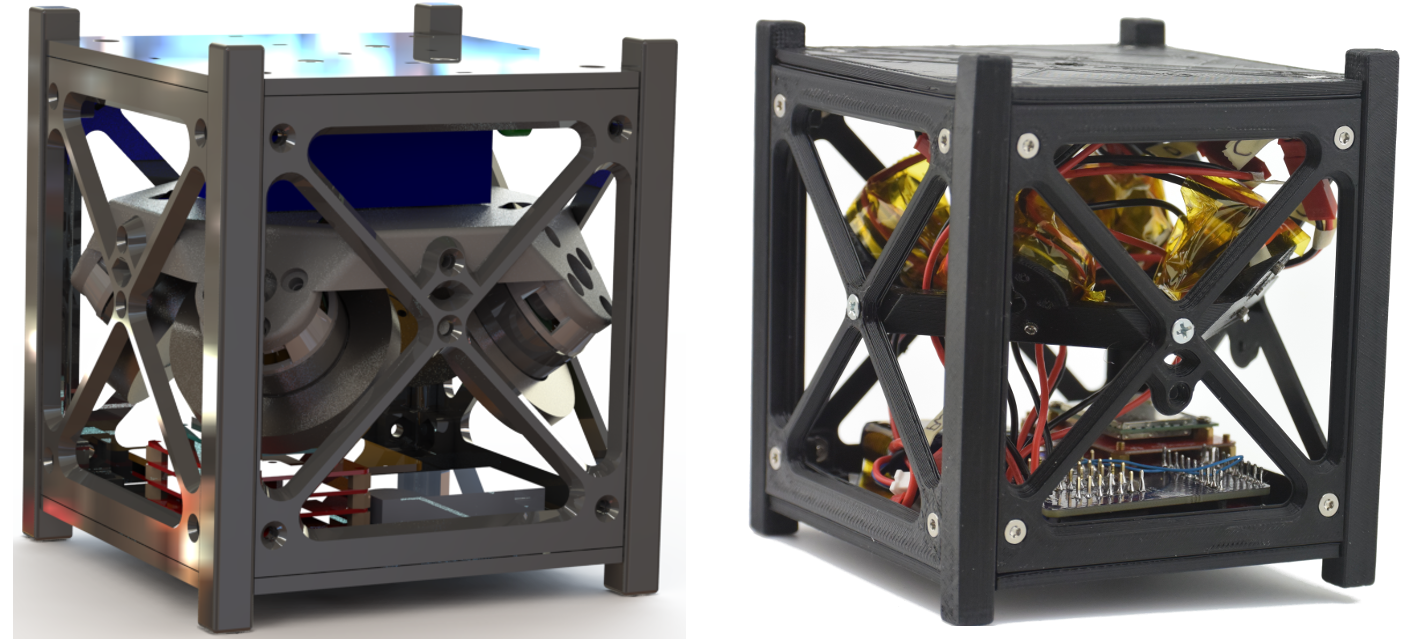
\includegraphics[width=0.7\linewidth]{20160224_195322.png}
  \caption{Reaction wheel ground test articles: a CAD render in SolidWorks, and the completed prototype.}
  \label{fig:rcs}
\end{figure}

\section{Controls Simulation and Design}
The controller for the reaction wheel system is a PI loop implemented on an Intel Edison with code written in Python. The Edison receives feedback from a 9-DoF IMU and sends signals via GPIO to the motors. The top-level controller design procedure was as follows:
\begin{enumerate}
\item Determine the transfer functions from dynamics analysis of free body diagrams of the system
\item Create simulation in GNU Octave
\item Design the controller using iterative testing (with comparisons to the model) and classical Bode techniques
\end{enumerate}
The transfer functions are determined with a dynamics analysis of the free body diagram, shown schematically for a single axis in Figure \ref{fig:FBD}. The forces acting on the cube are the torques created by the motors $T_i^0$, damping effects $b_1 \dot{\theta}_{cube}$, and spring effects $G_1 \theta_{cube}$. Summing the moments around the center of gravity gives the following equation:\\

\begin{equation}
\label{eq:moment}
\sum M_0^{+ \circlearrowleft} = I_{x,cube} \ddot{\theta}_{x,cube} = T^0_{Ax} + T^0_{Bx} - T^0_{Cx} - T^0_{Dx} + T^0_x - \dot{\theta}_{x,cube} - G_x \theta_{x,cube}
\end{equation}\\
	
Solving Eqn. \ref{eq:moment} so that $\theta_{cube}$ and its derivatives are on the left side, and the motor torques are on the right side, as well as setting the system to Standard Equilibrium Position (at SEP the input perturbations are set to zero) and substituting the torque-inertia relation:\\

\[
T^0_x = 0
\]
\[
T^0_{nx} = I_{rw}\ddot{\theta}_n\]\\

This gives us the following equation:\\
 
\[
I_{x,cube} \alpha_x + b_x \dot{\theta}_{x,cube} + G_x \theta_{x,cube} = \sin(45^{\circ}) I_{rw} (\ddot{\theta}_A + \ddot{\theta}_B -\ddot{\theta}_C - \ddot{\theta}_D)
\]\\	
Per the textbook definition of a transfer function we have the output of a system with respect to a single input, so all motors are set to zero except for one (A for this example) and apply a Laplace transform to the equation:\\

\[
\frac{I_{x,cube}}{\sin(45^{\circ}) I_{rw}} \theta_{x,cube} s^2 +
\frac{b_x}{\sin(45^{\circ}) I_{rw}} \theta_{x,cube} s +
\frac{G_x}{\sin(45^{\circ}) I_{rw}} \theta_{x,cube} = \theta_A s^2
\]\\
	
Finally moving $\theta_{cube}$ and $\theta_A$ to the left side of the equation and everything else to the right, gives us a transfer function:\\

\begin{equation}
\label{eq:xfer}
G_A(s)=\frac{\theta_{x,cube}(s)}{\theta_A(s)}=\frac{s^2}{\cfrac{I_{x,cube}}{\sin(45^{\circ}) I_{rw}}s^2 + \cfrac{b_x}{\sin(45^{\circ}) I_{rw}}s + \cfrac{G_x}{\sin(45^{\circ}) I_{rw}}}
\end{equation}\\
	
Using the transfer functions, given schematically for one axis by Eqn. \ref{eq:xfer} a simulation was created in GNU Octave which yielded step response plots shown in Figure \ref{fig:simulation}. The simulation will further aid in Bode analysis for the determination of stability margins. These relate the frequency response of the system to its time response. The margins can be adjusted with the use of a controller to affect the time response characteristics of the system. In the case of the ground test system the rise time for a $90^{\circ}$ step input should be under 1 second. 
\begin{figure}[h!]
  \centering
  \includesvg[width=0.35\linewidth]{FBD}
  \caption{Free Body Diagram of the CubeSat in the Cartesian x-axis.}
  \label{fig:FBD}
\end{figure}

\begin{figure}[h!]
  \centering
  {\footnotesize \includesvg[width=0.9\linewidth]{motor_torque}}
  \caption{CubeSat step response compared with singular motor response.}
  \label{fig:simulation}
\end{figure}

\begin{figure}[!ht]
 \centering
 {\includesvg[width=0.9\linewidth]{drop_test}}
 \caption{Time lapse of the CubeSat controller drop tower test. Initial roll impulse damped to 0 rad/s in approximately 1.9 s.}
 \label{fig:lapse}
\end{figure}

\begin{figure}[!ht]
 \centering
 {\footnotesize \includesvg[width=0.9\linewidth]{Gyro_Data_vs_Model}}
 \caption{Drop tower test 1-DoF gyro data for z-angular rates compared to the controller model.}
 \label{fig:drop_results}
\end{figure}

\section{Controller Testing and Results}
An exciting testing opportunity involves exploiting the high-quality $\mu$-gravity environment of Portland State University's Dryden Drop Tower (DDT) facility for free fall tests of the reaction wheel system. The Dryden Drop Tower, patterned on the 2.2 Second Drop Tower facility at NASA's Glenn Research Center in Cleveland, Ohio, is optimized for exceptionally fast drop turnaround times. The DDT is one of the most productive drop towers in the world for its class, with more than 5800 drops over its 6 year history. The DDT's 2.1 seconds of free-fall conditions provide unique opportunities for the observation of phenomena that are usually masked at the macro-scale in 1-g gravity fields. The relative quality of the $\mu$-gravity environment of a drop tower is very high compared to those offered by parabolic flights (generally $10^{-5}$ or $10^{-6}$-g for the drop tower compared to $10^{-1}$ or $10^{-2}$-g for a parabolic flight. In this high quality $\mu$-gravity the CubeSat attitude control can be tested in an environment similar to that of space (at least in an inertial sense). In the DDT the reaction wheel system testing program involved a random ( 25 \% duty cycle PWM) perturbing impulse followed by a command to damp this roll in the brief cinderella-like moment before the simulacrum of $\mu$-gravity disappears 2.1 seconds later. A time lapse plot showing the initial roll impulse and subsequent damping is presented in Figure \ref{fig:lapse}. On a qualitative examination of the simulated roll response compared to the experimental gyro rates from the IMU, the model appears to be quite accurate (in terms of the frequency and damping ratio), at least for this particular impulse. This is shown in Figure \ref{fig:drop_results}. The 0.1 s phase shift between the gyro data and the angular rates predicted by the simulation may be due to the discrete time lag of the physical controller, and also to the small ammount of damping by atmospheric drag. The gyro data is presented here in an unfiltered form. 

Following from the first test, an initial modicum of model validation allows us to continue with the model as the basis for further iterative controls testing. We plan to select a series of additional test points to formulate a more complete Bode diagram. This will require drop tests at several additional frequencies. Once the Bode diagram is completed a new model can be backed out, and the iterative controller design loop can be started anew. This work is in progress (as of August, 2016), and should be completed before the Oresat Critical Design Review in November 2016 which is concurrent with the next round of NASA ELaNa proposals.

\section{Acknowledgments}
We are indebted to PSU undergraduates Marie House, and Alex Farias, for their assistance with testing the prototype. We are further indebted to the PSU's Dryden Drop Tower Lab and the Lab for Interconnected Devices for their support both in fabricating and testing this prototype. We acknowlegde PSAS's faculty mentor, Andrew Greenberg, for his support and advice. Finally, we appreciate the support of the PSAS crowdfunders for helping to translate `citizen science' from a abstract ideal into a well realized reality, and for helping to translate some starry-eyed STEM student's dreams of space into Oregon's first orbital satellite.

\begin{thebibliography}{9}% maximum number of references (for label width)

\bibitem{Mahoney:15bk}
Mahoney, Erin. {\it CubeSat Launch Initiative: 50 CubeSats from 50 States in 5 Years.} NASA, April 9, 2015. http://www.nasa.gov/content/cubesat-launch-initiative-50-cubesats-from-50-states-in-5-years.\\

\bibitem{PSAS:15bk}
{\it Portland State Aerospace.} PSAS. Accessed February 25, 2016. http://psas.pdx.edu.\\

\bibitem{Cubesat:14bk}
The CubeSat Program, {\it Cal Poly SLO. CubeSat Design Specification Rev. 13.} San Luis
Obispo: California Polytechnic State University; 2014.\\

\bibitem{Oresat:15bk}
{\it Oregon Small Satellite Project.} GitHub. Accessed February 25, 2016. https://github.com/oresat.\\

\bibitem{Logan:08bk}
Logan, Jeffery. {\it Control and Sensor Development on a Four-Wheel Pyramidal Reaction Wheel Platform,} Master’s Thesis, California Polytechnic State University, San Luis Obispo, 2008.\\


\end{thebibliography}

\end{document}

